%!TEX root = ../Main.tex

% ------------------------------------------------------------------
\section{Fabrication of HTS Filter}
The HTS design was similar to the copper design except for a higher dielectric constant, E=24 and a thinner substrate h=0.5mm. The higher dielectric constant reduces the line length required to resonate at the same frequency. It also decreases the width of the 50 Ohm lines. The whole filter becomes much smaller and compact. The final design is shown in Figure~\ref{figure:design-hts-layout}.

\begin{figure}[ht]
\begin{center}
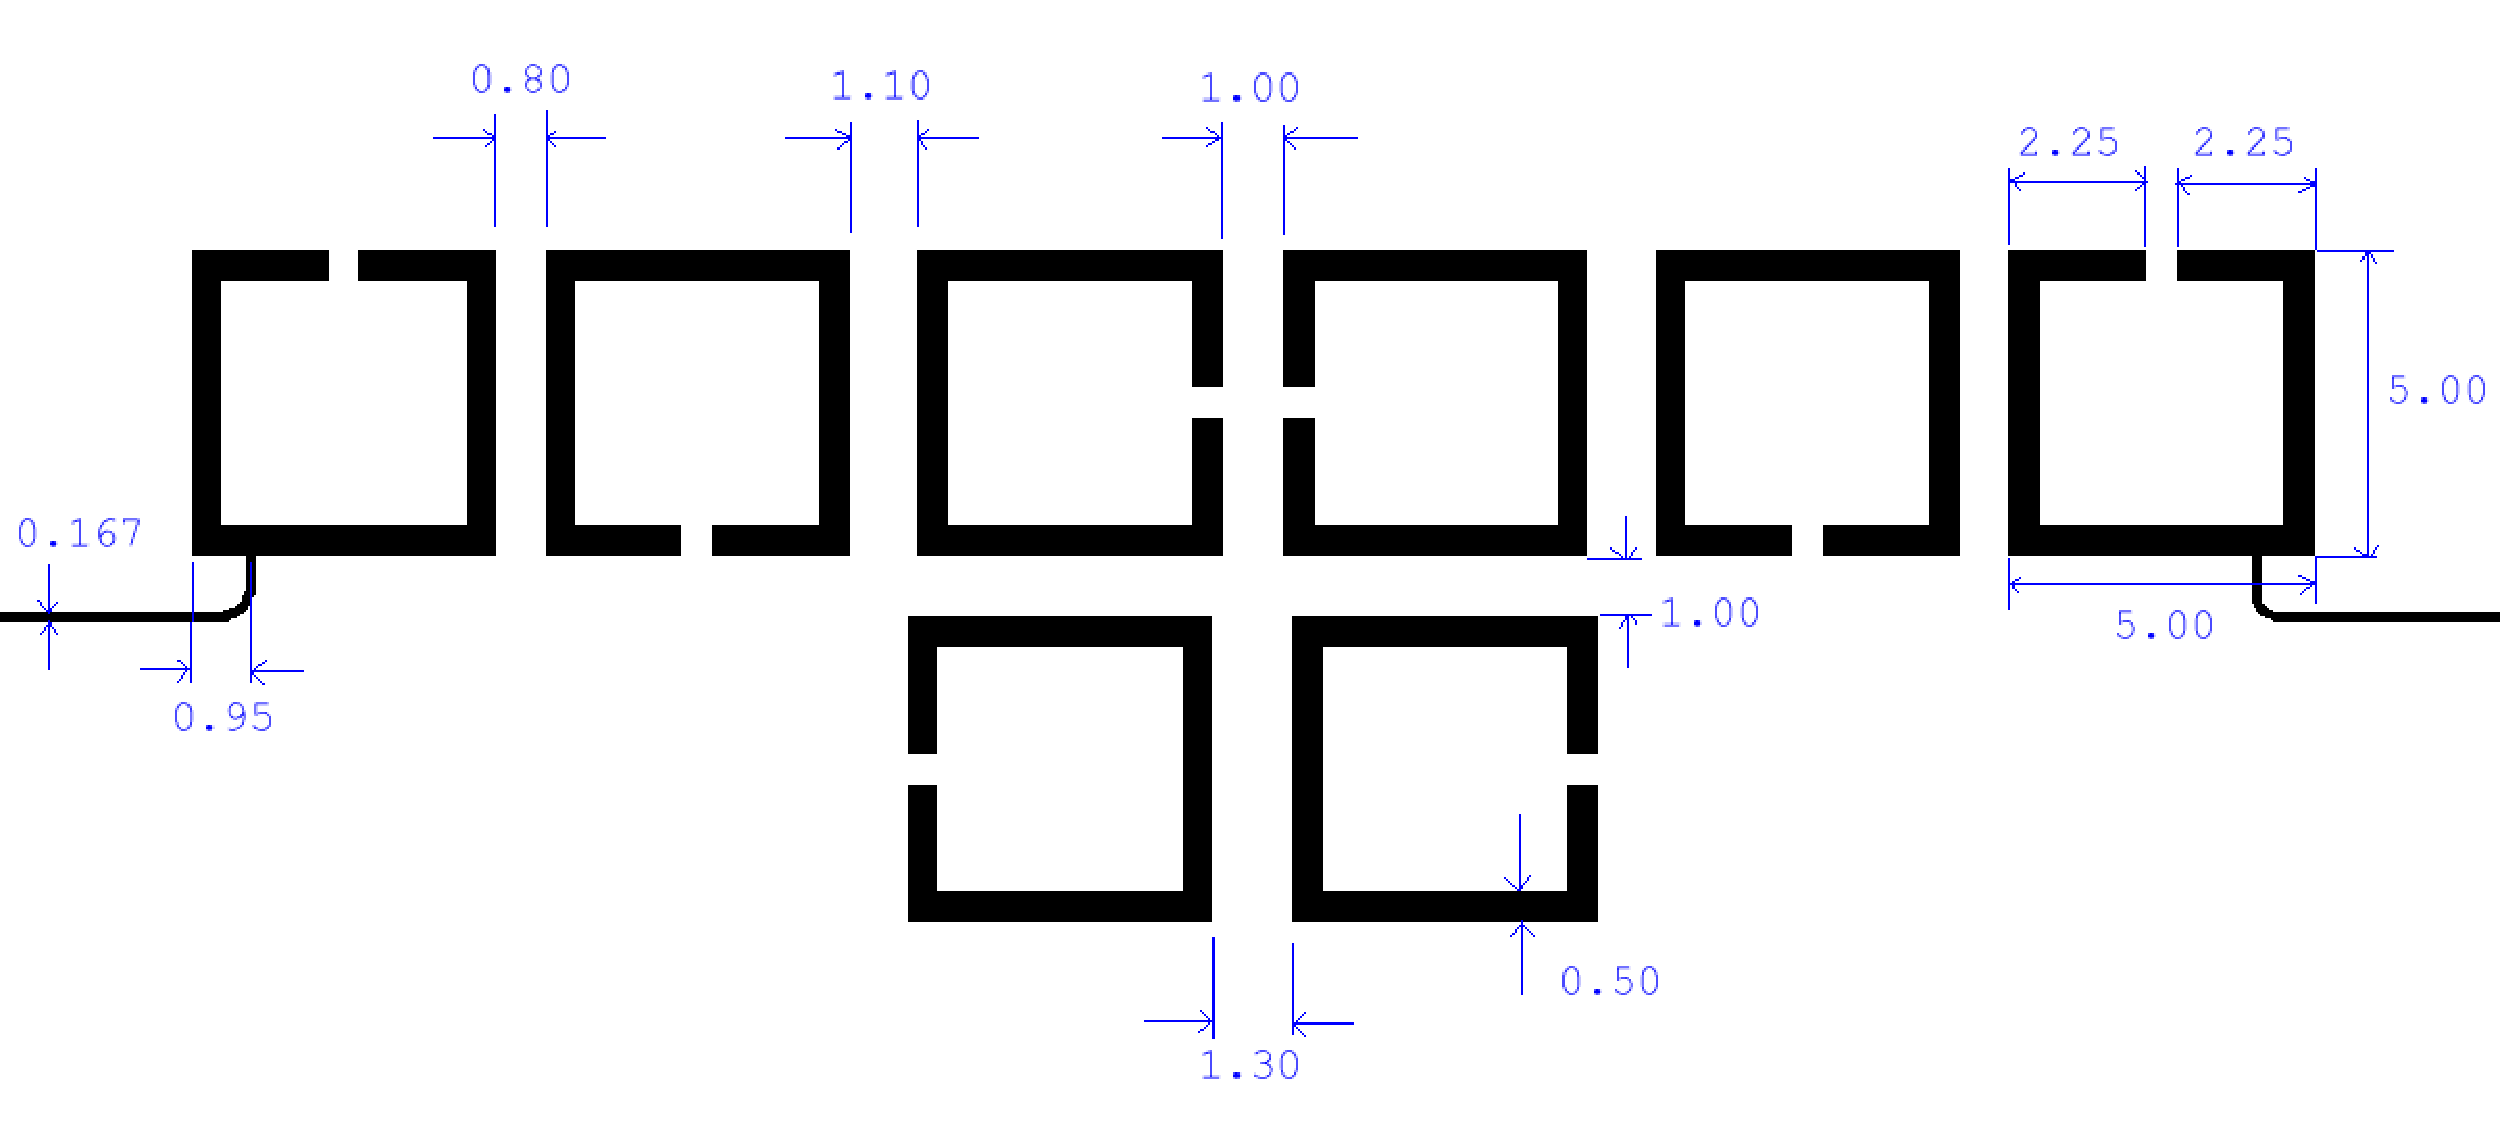
\includegraphics[scale=0.3]{fig/design-hts-layout.pdf}
\end{center}
\vspace{-1em}
\caption{HTS filter layout (dimensions in mm)}
\label{figure:design-hts-layout}
\end{figure}


% -----------------------------------------------------------------------------
\subsection{Fabrication}
The HTS material used was double sided YBCO thin film on a Lanthanum Aluminate substrate. Both sides were flashed with gold to provide a surface which could be soldered to. The HTS material is quite expensive so an effort was made to fit the filter on one half of a 50mm diameter wafer.

The filter was fabricated at the Linfield HTS lab and mounted in an existing box. The box was made from a Silicon Carbon Aluminate (SiCAl) base with copper sidewalls and a brass lid. The SiCAl base provides a good thermal expansion match with the LaAlO3 substrate and is also highly conductive. Silver paste was used to provide a good thermal and electrical contact between the ground plane and the base.

The SMA connectors used had a sliding center pin to account for the thermal contraction of the material. Indalloy 290 solder (In 97\% Ag 3\%) was used to attach the connector pins to the feed lines.

A picture of the final HTS filter is shown in Figure~\ref{figure:test-hts-open}. The picture shows a mess on the left hand feed line of the HTS filter. When the filter was first cooled this track was pulled from the substrate. Although the connector pins where supposed to slide with the contraction of the device, this did not happen. One possibility is that the pins were sticking in their housing as there was not enough mechanical strength in the YBCO-LaAlO3 bond to prevent it from breaking. Future designs will have the end of the feed several line widths wide to provide a stronger bonding surface.

\begin{figure}[ht]
\begin{center}
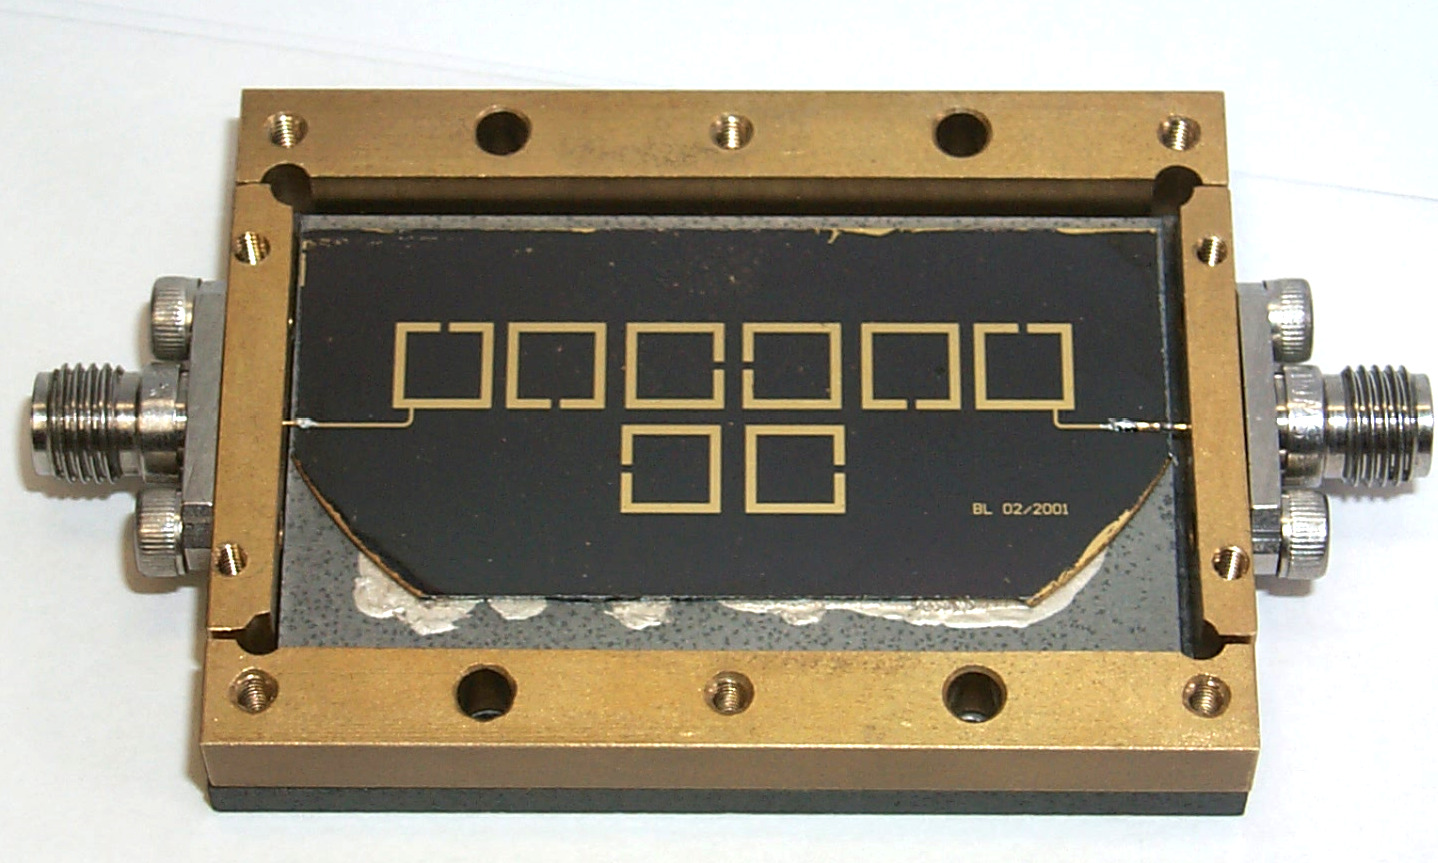
\includegraphics[scale=0.25]{fig/test-hts-open.jpg}
\end{center}
\vspace{-1em}
\caption{HTS Filter}
\label{figure:test-hts-open}
\end{figure}

\begin{figure}[ht]
\begin{center}
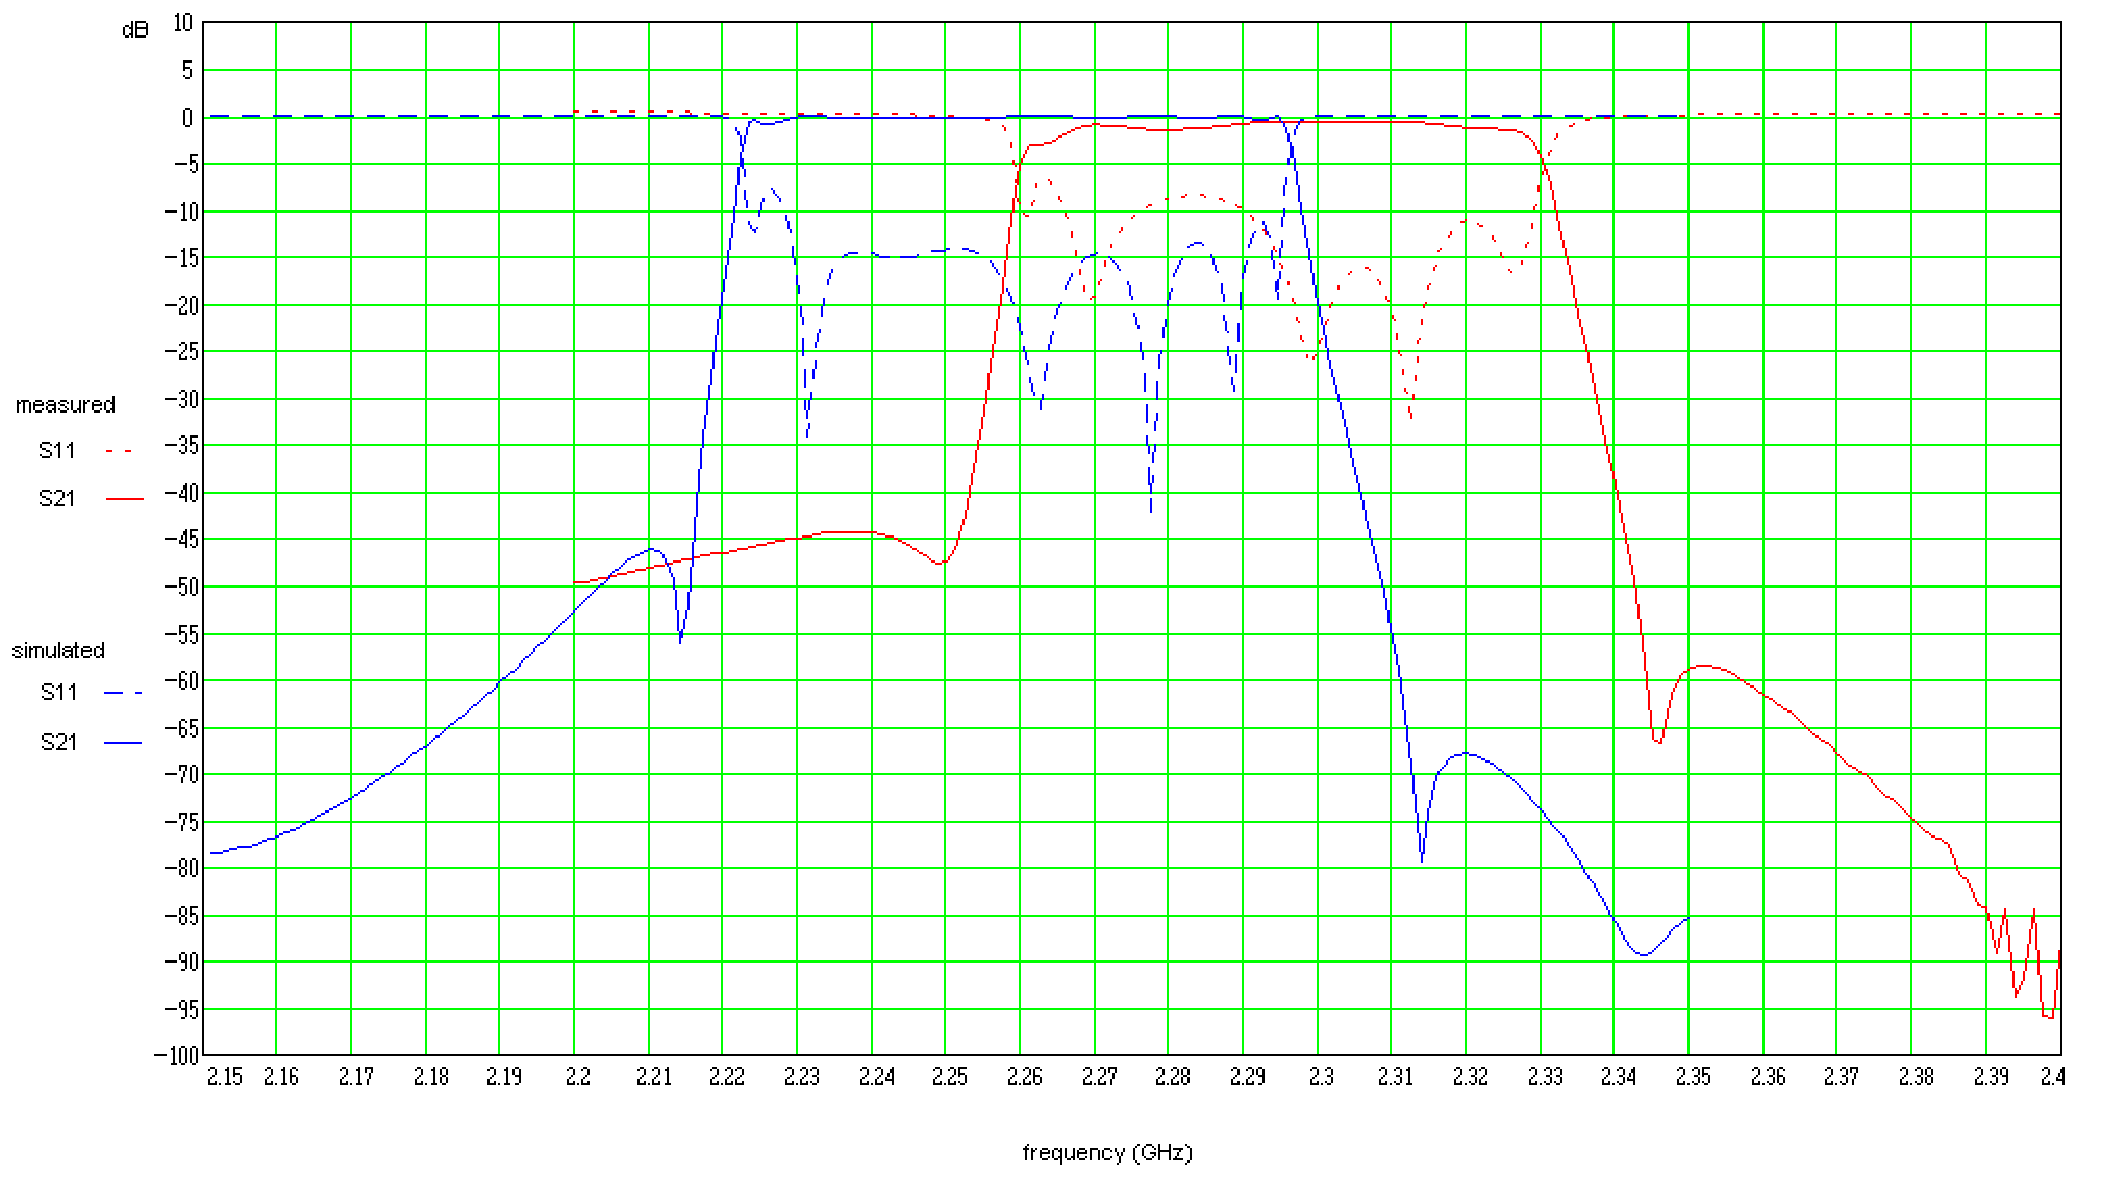
\includegraphics[scale=0.4]{fig/test-hts-response.pdf}
\end{center}
\vspace{-1em}
\caption{HTS filter response}
\label{figure:test-hts-response}
\end{figure}


% -----------------------------------------------------------------------------
\subsection{Result}
Once cooled, the filter gave the response shown in Figure~\ref{figure:test-hts-response}. The shape of the response was acceptable, withoug the rounding of the passband seen in the copper. The insertion loss in the center of the band was measured at 0.7dB.

There is a slight nick in the lower side of the passband of the simulated response, who's effects are also seen in the measured response. As mentioned earlier, although the separations of the resonators can be adjusted to give the coupling coefficient required by the filter synthesis tables, the filter synthesis tables to not account for non-adjacent couplings. This has caused the nick in the passband and also the asymmetry in the stop band. There will always be a degree of tuning required if perfect symmetry is desired.

This time, the filter response was 35MHz too high. A HTS film behaves slightly differently to how a perfectly conducting metal would~\cite{Shen:hts}. The simulator used does not take these effects into account though simulators are available which do. There is also a degree of uncertainty in the cooled dielectric constant of the material, it is often quoted as \emph{approximately} 24. 


% ------------------------------------------------------------------
\subsection{Tuning}
As with the copper filter the next step was to plant tuning screws in the box lid and attempt to clean up the response. Screws were placed into the fringe fields between the resonators and at the resonator ends to adjust the center frequency.

There was a difficulty in adjusting the tuning screws when the filter was in the sealed vacuum dewar. The first attempted solution to this problem was to screw a test device onto a copper block. The base of the block was then immersed in liquid nitrogen leaving the filter above the surface. This provided a moderate cooling rate for the filter as well as easy access to the screws. Unfortunately moisture had condensed from the atmosphere and froze onto both the filter body and the part of the block which was above the nitrogen.

As the YBCO HTS film is susceptible to moisture, this procedure was deemed unusable as the device would be ruined when it was re-warmed and the ice liquefied. It is important to note that the filter box is not sealed as there are gaps in the body to account for the thermal contraction of the copper walls.

The next solution was to drill a set of holes in a perspex dewar lid and insert rubber bungs with screwdrivers set through the middle. A picture of the setup used is shown in Figure~\ref{figure:test-hts-fridge}.

As the bung cannot be tilted too far for risk of breaking the vacuum seal, there were two separate screwdrivers installed so all screws could be reached.

Even with vacuum grease sealing the rubber-perspex and rubber-screwdriver interfaces there is a small amount of air leakage though it is not problematic. The white circle in the center of the cold plate consists of nitrogen and water vapor which has leaked into the dewar and frozen.

Although the tuning setup was successful, the range of tuning possible was inadequate to improve the filter response. The zero on the low side of the response could be deepened slightly and the passband ripples smoothed out a little. The number of tuning variables ( number of screws) is large enough to make the tuning process  time consuming and more a process of trial and error than anything else.

More importantly, the center frequency of the resonators was found to be tunable by less than 5MHz or so, which was insufficient to correct the 35MHz difference in center frequency.

\begin{figure}[ht]
\begin{center}
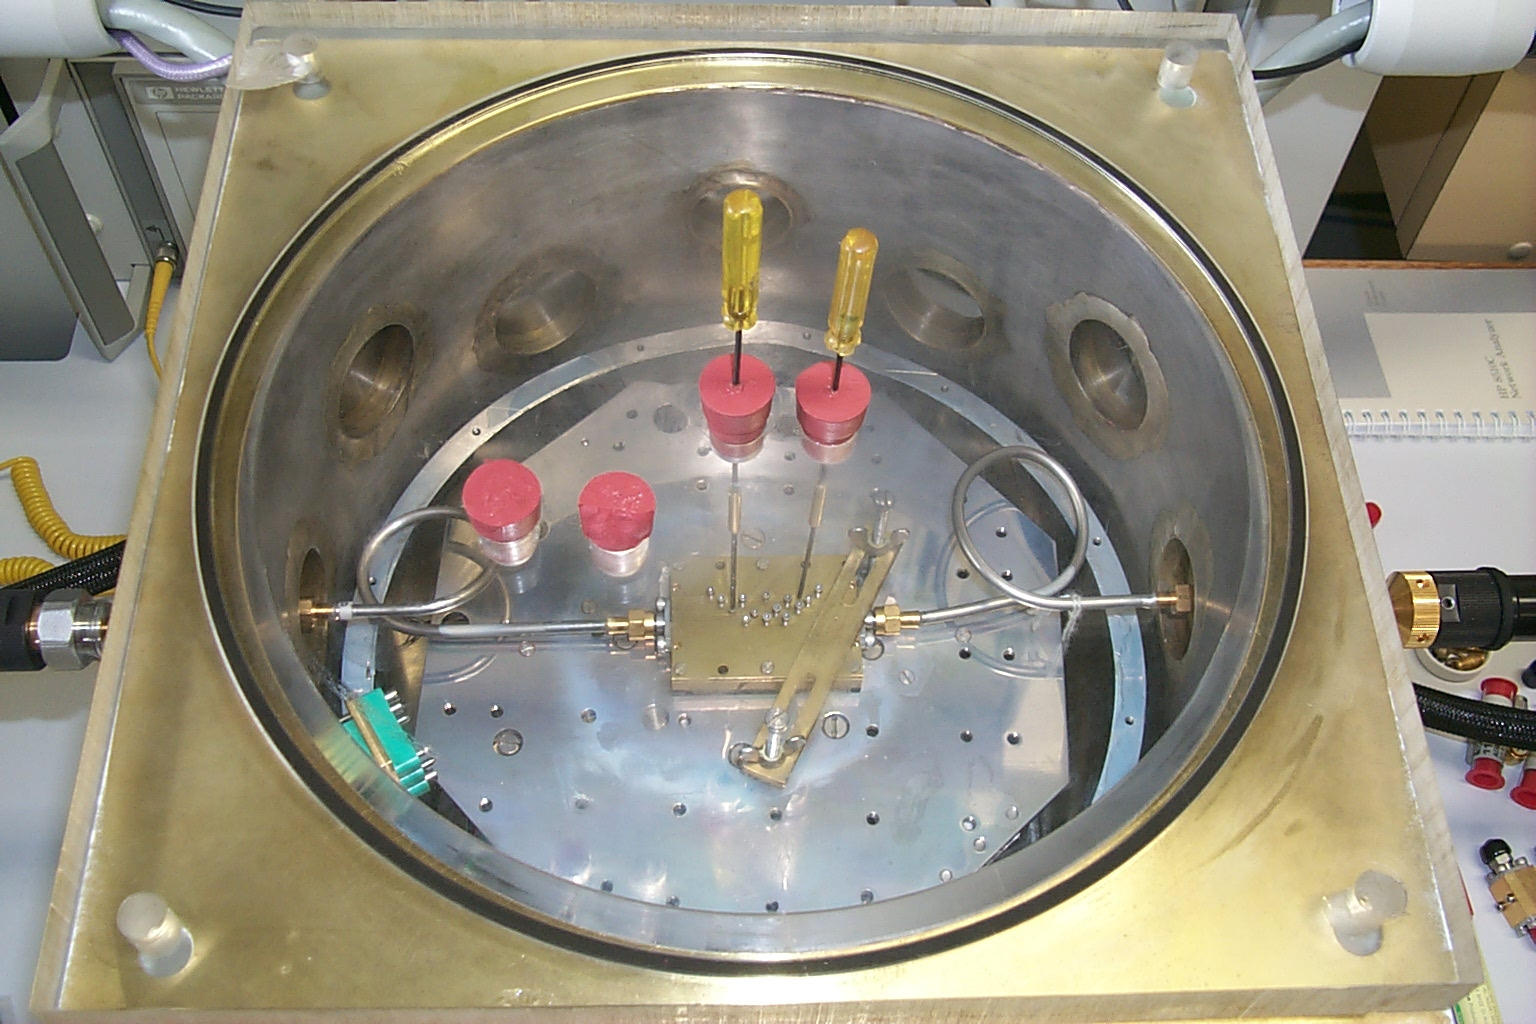
\includegraphics[scale=0.2]{fig/test-hts-fridge.jpg}
\end{center}
\vspace{-1em}
\caption{HTS filter in fridge}
\label{figure:test-hts-fridge}
\end{figure}

